\section{需求分析}

一个压缩解压实用程序,要读取输入文件,压缩之后写出输出文件,并可以把压缩文件解压还原成原来的文件。由此我们要实现这两个功能:
\begin{itemize}
\item 对文件进行编码
\item 对文件进行解码
\end{itemize}

\subsection{前缀码}

假定我们希望压缩一个十万字符的文件。表 \ref{basetable} 给出了文件中所出现的字符和它们的出现频率。

如表\ref{basetable}。一个 100 000 个字符的文件,只包含 a--f 6个不同字符,频率如此。如果为每个字符指定一个 3 位的码字,则文件编码长度为 300 000 位。但如果使用变长编码,就可以下降到 224 000 位。

\begin{table}[h]
\centering
\caption{\label{basetable}一个字符编码问题}
\begin{tabular}{|l|cccccc|}\hline
 & a & b & c & d & e & f \\\hline
频率(千次) & 45 & 13 & 12 & 16 & 9 & 5 \\
定长编码 & 000 & 001 & 010 & 011 & 100 & 101 \\
变长编码 & 0 & 101 & 100 & 111 & 1101 & 1100 \\\hline
\end{tabular}
\end{table}

本来,如果采用定长编码,这个文件需要 300 000 个二进制位(bit) 来表示。换用表 \ref{basetable} 给出的变长编码之后,则只需要
\[ (45\cdot 1 + 13\cdot 3 + 12\cdot 3 + 16\cdot 3 + 9\cdot 4 + 5\cdot 4)\cdot 1 000 = 224 000\,{\mathrm{bit}} \]
就能表示该文件,相比节约了 20\% 的空间。实际上,可以证明,这就是该文件的最优字符编码。

这里我们只考虑前缀码,即没有任何字符是其他码字的前缀。任何二进制字符码的编码过程都很简单,只要将每个字符的码字连接起来即可完成文件编码。前缀码的作用是简化解码过程。由于没有码字是其他码字的前缀,编码文件的开始码字是无歧义的。可以简单地识别出开始码字,将其转换回原字符,然后对剩余部分重复此过程即可。

\subsection{构造 Huffman 编码}

哈夫曼编码 (Huffman coding),又译霍夫曼编码、哈弗曼编码、赫夫曼编码,是一种古老的压缩算法,它是一种基于最小冗余编码的压缩算法 \cite{maic}。最小冗余编码是指,如果知道一组数据中符号出现的频率,就可以用相应的的位数来表示符号从而减少数据需要的空间。David A. Huffman \cite{huffman} 设计这样了一个贪心算法来构造最优前缀码。

下面给出该算法的伪代码。假定 $C$ 是一个 $n$ 个字符的集合,其中每个字符 $c\in C$ 都是一个对象,其属性 $c.freq$ 表示字符的出现频率,事先已经计算好。算法自底向上构造出对应最优编码的二叉树 $T$。它从 $n$ 个叶节点开始,执行 $n-1$ 次合并操作,创建出最终的二叉树。$Q$ 是一个有序存储结构,每次取出其中 $freq$ 属性最小的两个对象进行合并。合并之时,得到的新对象的频率则设为原来两个对象频率之和。

\begin{quote}
\begin{codebox}
\Procname{\proc{Huffman}($C$)}
\li $n = |C|$
\li $Q = C$
\li \For $i = 1$ \To $n-1$ \Do
\li   为 $z$ 分配存储空间
\li   $z.left = x = $ \proc{Extract-Min}($Q$)
\li   $z.right = y = $ \proc{Extract-Min}($Q$)
\li   $z.freq = x.freq + y.freq$
\li   \proc{Insert}($Q$, $z$)
    \End
\li \Return \proc{Extract-Min}($Q$)
\label{Huffman-pc}\index{\proc{Huffman}}
\end{codebox}
\end{quote}

算法运行速度取决于 $Q$ 的实现。一般地情况下,使用 Fibonacci 堆可以得到
\[ O(1) + O(n-1)\cdot (2O(\lg n) + O(1)) = O(n\lg n)\]
的时间复杂度,但相应的实现比较复杂,可以成为另一个课题讨论\footnote{实际上,使用 van Emde Boas 树还可以进一步优化成 $O(n\lg\lg n)$,这里不再讨论。}。

这里简化问题,使用一个数组存储,每次插入之后进行一次增序排序(使用快速排序),每次取出最前面两个元素即可,而时间复杂度就退化成了
\[ O(1) + O(n-1)\cdot (2O(1) + O(n\lg n)) = O(n^2\lg n)\]

实际上,由于 $n$ 是字符集数量,这个值一般是个常数,为 256。在实际运行中,这样小的规模中,$O(n\lg n)$ 的优势并不比 $O(n^2\lg n)$ 好多少。这并不是一个严重的问题,相对于庞大的数据量来说,符号数造成的影响小到可以忽略。

图 \ref{clrs_huffman} 是对表 \ref{basetable} 给出的频率执行 Huffman 算法的过程。每一部分显示了 $Q$ 中的内容,且已有递增序。每个步骤中,频率最低的两棵树进行合并。叶结点用矩形表示,包含一个字符及其频率。内部结点用圆圈表示,包含其孩子结点频率之和。结点指向左孩子的边标记为 0,指向右孩子的边标记为 1。一个字母的码字对应从根到其叶结点的路径上的边标记序列。(a)初始集合有 $n=6$ 个结点,每个结点对应一个字母。 (b)--(e) 为中间步骤。(f) 是最终的编码树。

\begin{figure}[htbp]
\centering
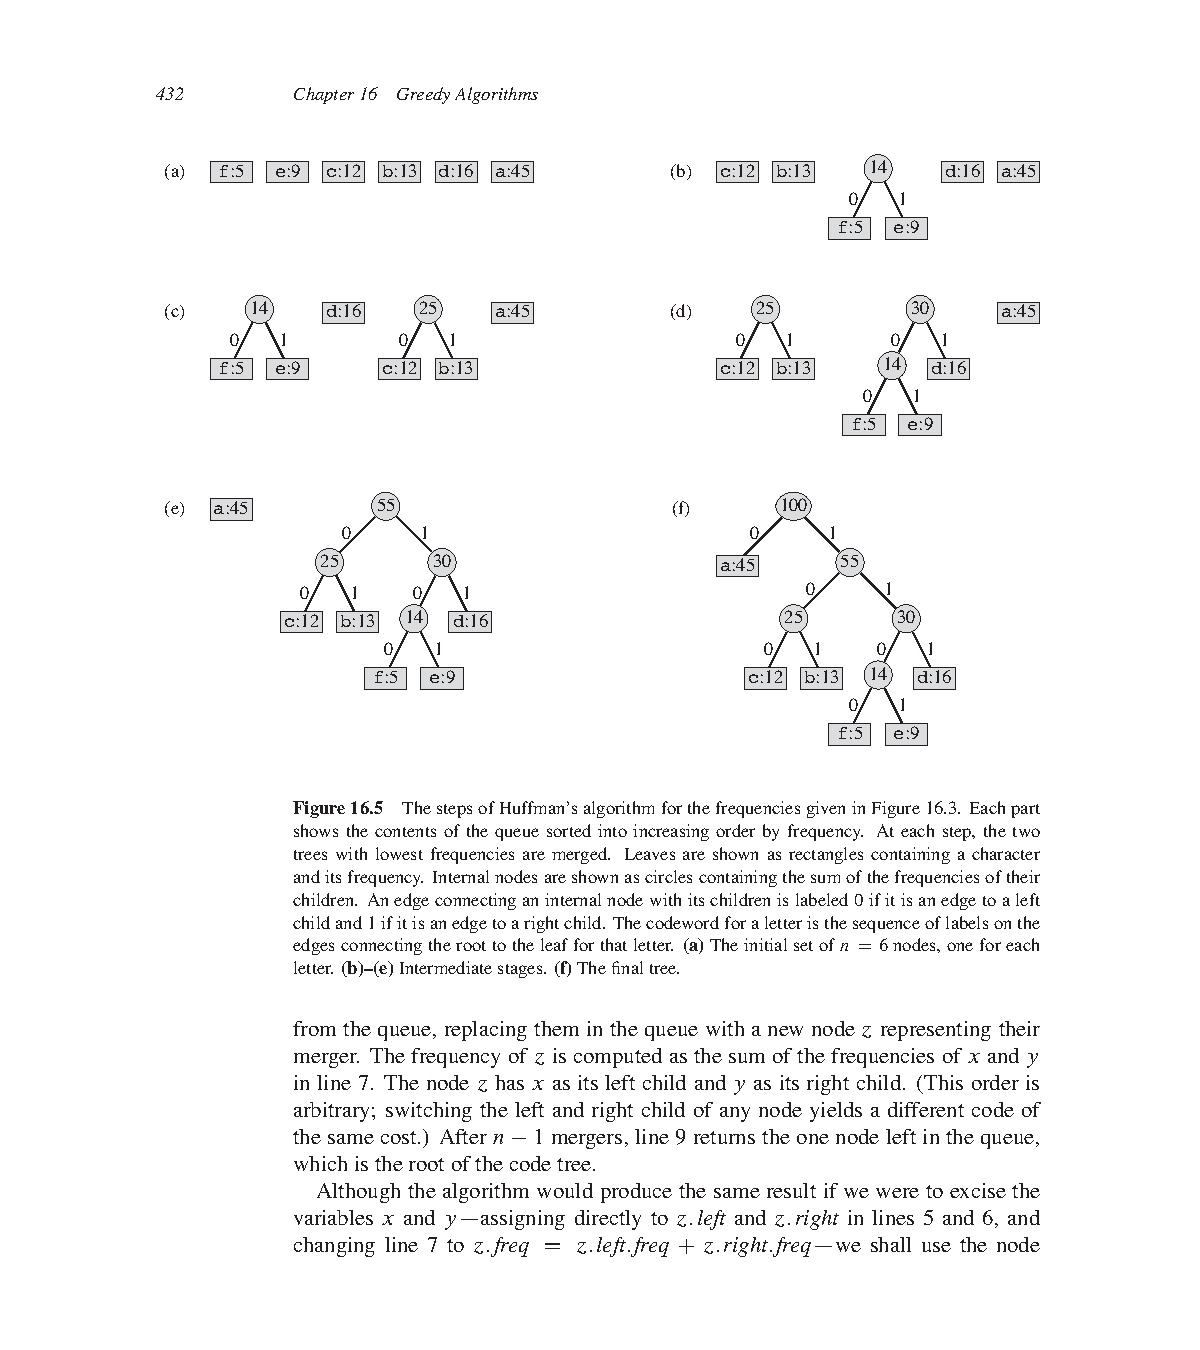
\includegraphics[trim=28mm 102mm 22mm 24mm,clip]{image/clrs_huffman.pdf}
\caption{\label{clrs_huffman}对表 \ref{basetable} 给出的频率执行 Huffman 算法的过程 \cite{clrs}}
\end{figure}

对前文给出的例子,Huffman 算法的执行过程如图 \ref{clrs_huffman} 所示。字母表包含 6 个字母所以初始 $n=6$,需要 5 个合并步骤构造二叉树。最终的二叉树表示最优前缀码。每个字母的码字为根节点到该字母叶结点的简单路径上边标签的序列。

\subsection{编码和解码}

由于所有文件都是二进制存放的,所以我这里不讨论文件编码\footnote{通常的文件编码最小单位都是字节(byte),包括 ASCII 和 GB 定长编码和 UTF-8 变长编码,这些都是用作通常存储的非压缩编码。}问题,将中文字符和西文字符都看做字节,减少问题的复杂度。由于我们不安排编码,所以压缩解压后文件编码如原文一致。这样理论上也可以压缩图片、音乐甚至视频等非文本文件。所以我们以二进制方式读入写出文件。

编码时,读入文件,从头到尾扫描一遍,统计每个字符(符号)的出现次数(频率)。然后,依据该频率统计结果,构造一棵 Huffman 树,并依此树生成一个编码表。写出该编码表。再次扫描文件,根据 Huffman 树编码每个字符,并写出到文件。

解码时,读入文件开始部分的编码表,依此构建 Huffman 树。接着读入剩余字符,根据 Huffman 树解码每个字符,并写出到文件。
